\documentclass{ntuaclass} % η κλάση του εγγαφου
\usepackage{lipsum} % το χρησιμοποιώ για dummy-text

% ο φάκελος με τις εικόνες
\graphicspath{{./images/}}

% το αρχείο με τις βιβλιογραφικές αναφορές  uncomment για βιβλιογραφία
%\bibliography{bibliography.bib} 

% ο τίτλος του εγγράφου
\Type{τέστ και τεστ}
\Title{Τίτλος}
\Eks{7}
\Mathima{Ρευστά}
\Onomatepwnumo{\en{Kellaris}}
\Armhtrwou{02117010}
\Omada{7} % προαιρετικό 
\Hmeromhnia{\today}

% διορθώνει τα μεταδεδομένα του αρχείου
\fixmetadata

%αλλαγή τίτλου του κεφαλαίου π.χ. ερώτημα
%\setchapname{Ερώτημα} uncomment για χρήση

% χρήση της εντολής ώστε να κάνει compile μόνο το κεφάλαιο που αλλάξαμε
%\includeonly{chapters/3rdchapter} uncomment για χρήση

\begin{document}

% δημιουργεί το εξώφυλλο
\ntuatitle

%δημιουργεί τον πίνακα περιεχομένων με σωστό τρόπο
\maketoc

% μια καλή πρακτική είναι κάθε κεφάλαιο να γράφεται σε ξεχωριστό αρχείο
\section{Πρώτο δοκιμαστικό κεφάλαιο}
\en{\lipsum}
\cite{bowenspaper}
\begin{figure}[tbp]
    \centering
    \en{% GNUPLOT: LaTeX picture with Postscript
\begingroup
  \makeatletter
  \providecommand\color[2][]{%
    \GenericError{(gnuplot) \space\space\space\@spaces}{%
      Package color not loaded in conjunction with
      terminal option `colourtext'%
    }{See the gnuplot documentation for explanation.%
    }{Either use 'blacktext' in gnuplot or load the package
      color.sty in LaTeX.}%
    \renewcommand\color[2][]{}%
  }%
  \providecommand\includegraphics[2][]{%
    \GenericError{(gnuplot) \space\space\space\@spaces}{%
      Package graphicx or graphics not loaded%
    }{See the gnuplot documentation for explanation.%
    }{The gnuplot epslatex terminal needs graphicx.sty or graphics.sty.}%
    \renewcommand\includegraphics[2][]{}%
  }%
  \providecommand\rotatebox[2]{#2}%
  \@ifundefined{ifGPcolor}{%
    \newif\ifGPcolor
    \GPcolortrue
  }{}%
  \@ifundefined{ifGPblacktext}{%
    \newif\ifGPblacktext
    \GPblacktexttrue
  }{}%
  % define a \g@addto@macro without @ in the name:
  \let\gplgaddtomacro\g@addto@macro
  % define empty templates for all commands taking text:
  \gdef\gplbacktext{}%
  \gdef\gplfronttext{}%
  \makeatother
  \ifGPblacktext
    % no textcolor at all
    \def\colorrgb#1{}%
    \def\colorgray#1{}%
  \else
    % gray or color?
    \ifGPcolor
      \def\colorrgb#1{\color[rgb]{#1}}%
      \def\colorgray#1{\color[gray]{#1}}%
      \expandafter\def\csname LTw\endcsname{\color{white}}%
      \expandafter\def\csname LTb\endcsname{\color{black}}%
      \expandafter\def\csname LTa\endcsname{\color{black}}%
      \expandafter\def\csname LT0\endcsname{\color[rgb]{1,0,0}}%
      \expandafter\def\csname LT1\endcsname{\color[rgb]{0,1,0}}%
      \expandafter\def\csname LT2\endcsname{\color[rgb]{0,0,1}}%
      \expandafter\def\csname LT3\endcsname{\color[rgb]{1,0,1}}%
      \expandafter\def\csname LT4\endcsname{\color[rgb]{0,1,1}}%
      \expandafter\def\csname LT5\endcsname{\color[rgb]{1,1,0}}%
      \expandafter\def\csname LT6\endcsname{\color[rgb]{0,0,0}}%
      \expandafter\def\csname LT7\endcsname{\color[rgb]{1,0.3,0}}%
      \expandafter\def\csname LT8\endcsname{\color[rgb]{0.5,0.5,0.5}}%
    \else
      % gray
      \def\colorrgb#1{\color{black}}%
      \def\colorgray#1{\color[gray]{#1}}%
      \expandafter\def\csname LTw\endcsname{\color{white}}%
      \expandafter\def\csname LTb\endcsname{\color{black}}%
      \expandafter\def\csname LTa\endcsname{\color{black}}%
      \expandafter\def\csname LT0\endcsname{\color{black}}%
      \expandafter\def\csname LT1\endcsname{\color{black}}%
      \expandafter\def\csname LT2\endcsname{\color{black}}%
      \expandafter\def\csname LT3\endcsname{\color{black}}%
      \expandafter\def\csname LT4\endcsname{\color{black}}%
      \expandafter\def\csname LT5\endcsname{\color{black}}%
      \expandafter\def\csname LT6\endcsname{\color{black}}%
      \expandafter\def\csname LT7\endcsname{\color{black}}%
      \expandafter\def\csname LT8\endcsname{\color{black}}%
    \fi
  \fi
    \setlength{\unitlength}{0.0500bp}%
    \ifx\gptboxheight\undefined%
      \newlength{\gptboxheight}%
      \newlength{\gptboxwidth}%
      \newsavebox{\gptboxtext}%
    \fi%
    \setlength{\fboxrule}{0.5pt}%
    \setlength{\fboxsep}{1pt}%
\begin{picture}(5660.00,5660.00)%
    \gplgaddtomacro\gplbacktext{%
      \csname LTb\endcsname%%
      \put(616,652){\makebox(0,0)[r]{\strut{}$-0.4$}}%
      \csname LTb\endcsname%%
      \put(616,1277){\makebox(0,0)[r]{\strut{}$-0.2$}}%
      \csname LTb\endcsname%%
      \put(616,1902){\makebox(0,0)[r]{\strut{}$0$}}%
      \csname LTb\endcsname%%
      \put(616,2527){\makebox(0,0)[r]{\strut{}$0.2$}}%
      \csname LTb\endcsname%%
      \put(616,3152){\makebox(0,0)[r]{\strut{}$0.4$}}%
      \csname LTb\endcsname%%
      \put(616,3777){\makebox(0,0)[r]{\strut{}$0.6$}}%
      \csname LTb\endcsname%%
      \put(616,4402){\makebox(0,0)[r]{\strut{}$0.8$}}%
      \csname LTb\endcsname%%
      \put(616,5027){\makebox(0,0)[r]{\strut{}$1$}}%
      \csname LTb\endcsname%%
      \put(728,448){\makebox(0,0){\strut{}$-10$}}%
      \csname LTb\endcsname%%
      \put(1872,448){\makebox(0,0){\strut{}$-5$}}%
      \csname LTb\endcsname%%
      \put(3016,448){\makebox(0,0){\strut{}$0$}}%
      \csname LTb\endcsname%%
      \put(4159,448){\makebox(0,0){\strut{}$5$}}%
      \csname LTb\endcsname%%
      \put(5303,448){\makebox(0,0){\strut{}$10$}}%
    }%
    \gplgaddtomacro\gplfronttext{%
      \csname LTb\endcsname%%
      \put(3015,142){\makebox(0,0){\strut{}$\textrm{τεστ} \quad \frac{\textmu}{x}$}}%
      \csname LTb\endcsname%%
      \put(4438,4844){\makebox(0,0)[r]{\strut{}$sin(x)/x$}}%
      \csname LTb\endcsname%%
      \put(3015,5333){\makebox(0,0){\strut{}$\textrm{test}$}}%
    }%
    \gplbacktext
    \put(0,0){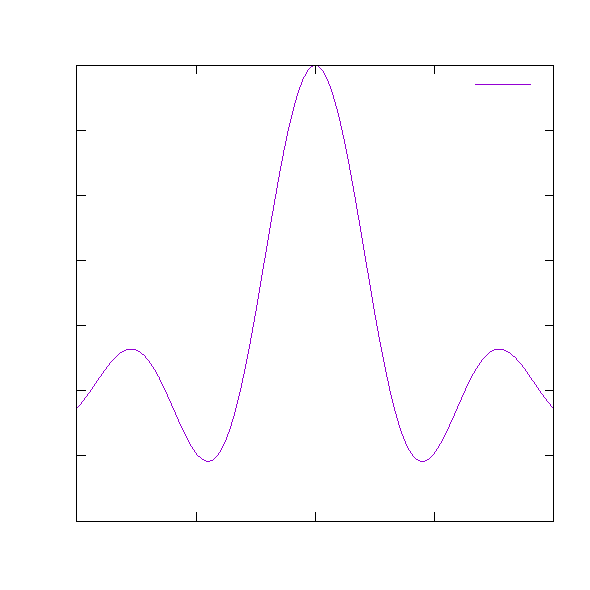
\includegraphics[width={283.00bp},height={283.00bp}]{gplot_example}}%
    \gplfronttext
  \end{picture}%
\endgroup
}
    \caption{Ένα διάγραμμα με \en{gnuplot}}
\end{figure}

\chapter{\texorpdfstring{Δοκιμαστικό κεφάλαιο με εικόνα \en{svg}}{Δοκιμαστικό κεφάλαιο με svg}}
\section{πρώτη ενότητα}
\en{\lipsum[1-2]}
\svg{images/ress.pdf_tex}{Δοκιμαστικός υπότιτλος}{1}
\section{άλλη μια ενότητα}
\en{\lipsum[3-4]}
\section{\texorpdfstring{Kεφάλαιο με αγγλικά στον τίτλο και \en{pdf}}{Kεφάλαιο με αγγλικά στον τίτλο και pdf}}
\pdf{a3.pdf}{\en{testcaption}}{2}
\subsection{τελευταία ενότητα}
\en{\lipsum}
\begin{figure}[tbp]
\centering
\begin{tikzpicture}
    \begin{axis}[
    siunitxlabels,
    legend style={minimum width=8 cm},
    xmin=0,xmax=4000,
    ymin=0,ymax=750,
    xtick={0,500,1000,1500,2000,2500,3000,3500,4000},
    ytick={0,150,300,450,600,750},
    xlabel={Απόσταση \en{m}},
    ylabel={Συγκέντρωση $μg/m^3$},
    legend pos=north east,
    ymajorgrids=true,
    xmajorgrids=true,
    grid style=dashed,
    width=0.9\textwidth,
    height=10cm
    ]
    \addplot[color=blue,no marks]  
      table[x=Distance, y=Concentration ,col sep=comma]
      {plots/5_0.2_0.77_0.24.csv };

    \addplot[color=red,no marks]  
      table[x=Distance, y=Concentration ,col sep=comma]
      {plots/10_0.2_0.77_0.24.csv };

    \addplot[color=green,no marks]  
      table[x=Distance, y=Concentration ,col sep=comma]
      {plots/15_0.2_0.77_0.24.csv };
    \addlegendentry{\en{H = 5m - $z_0 = 0.2m$ - bowen = 0.77 - albedo = 0.16}}
    \addlegendentry{\en{H = 10m - $z_0 = 0.2m$ - bowen = 0.77 - albedo = 0.16}}
    \addlegendentry{\en{H = 15m - $z_0 = 0.2m$ - bowen = 0.77 - albedo = 0.16}}
    \end{axis}
  \end{tikzpicture}
    \caption{Γράφημα συγκεντρώσεων με παράμετρο το ύψος καμινάδας}
  \label{fig:default}
\end{figure}
\en{\lipsum}

% uncomment για βιβλιογραφία

%\addcontentsline{toc}{chapter}{Βιβλιογραφία}
%\printbibliography

\end{document}